% Include Contributions page
\chapter{Plan of Work \& Project Management}

\section{Report Coordination}
\subsection{Breaking Up The Report}
As every group member is working on our project, it was important to ensure that every group member also worked on the report. However, it can be difficult to dole out responsibilities on something like this while ensuring fairness in terms of amount of research and work required. It seemed natural to divide up the the report based on each of our group member's strengths and the piece of our application that they would actually be working on themselves--that is, if a group member would be more responsible for front end aspects of our website, they should be the one to write about user interface specification. Such a division should allow for the highest quality of discussion on each aspect of specification in our report. Thus, we decided on the following break up for system specifications: \\
\begin{itemize}
\item{\textbf{Jeff Rabinowitz} - Jeff, being most familiar with finance and having broad general knowledge on software systems, took responsibility for defining things usch as customer requirements and system architecture.}
\item{\textbf{Nick Palumbo} - Nick's skills lie in programming and team management, and, as such, he took responsibility for detailing functional requirements and project management.}
\item{\textbf{Eric Cuiffo} - Eric is a talented designer and took responsibility for describing our user interface specification and design, including creating mock-ups and ease of use discussion.}
\item{\textbf{Dario Rethage} - Dario has worked intensively on website development before and also has a knack for design, so he helped Eric with user interface design along with defining our plan of work and describing project coordination.}
\item{\textbf{Val Red} - Val, good with databases and other ways of a system interfacing with external sources, was given the role of discussing our domain and class models for our system.}
\item{\textbf{Jeff Adler} - Jeff knows the nitty-gritty, low-level aspects of system and software development and was responsible for discussing subsystems and test design.}
\end{itemize}
It's important to note that this does not perfectly represent each members contributions, and that many sections had overlapping of team members. Sections that involved mock-ups and diagrams in particular were developed by several members overseen by the people given the responsibility as stated above. Pieces of the report not mentioned above were worked on by multiple or all of our members. The exact breakdown of contributions is given below in the section "Report 2 Contributions". \\

\subsection{Compiling The Report}
In order to ensure consistency, various venues of communication were opened: a group forum, group MMS, and collaborative online documents. Each member was asked to continually update the group on their progress and a synposis on the discussion they were including. Thus, the contributions of the members could be policed. In general, Jeff Rabinowitz and Nick Palumbo were responsible for ensuring everyone was doing their share of the work and that deadlines were being met. However, no decisions were made without the consent of the group; it was just necessary to have someone to make sure everything was running smoothly. Nick typically divided up labor and set deadlines, and Jeff kept an open dialogue with each member on their progress. \\

A single styling document was created which defined formatting standards (color, spacing, font, etc.) across the entire document and applied to each piece of the report, which guaranteed that all these aspects were held constant throughout. For each report submission: with enough time in advance of the deadline, each member submitted their piece of the report and Jeff Rabinowitz, being the group expert on Latex (used to create this report), proofread their formatting and syntax to ensure no compiling errors and consistency. He then submitted the final report to Nick who looked over the report to confirm the quality of each member's work and to ensure completeness of all topics covered. Each group member was responsible for the completeness of their own sections and would be notified of any deficiencies. Ultimately, Nick submitted the finalized report to the Sakai drop box. \\

\subsection{Issues}
 I (Nick) asked each group member to explain their experience on the coordination of the report, any praise or criticism they had for the fellow members, and any issues that were encountered:

\subsubsection{Nick Palumbo}
In general, I was satisfied with the coordination of our group. The only concern was that we occasionally struggled with deadlines. As only Jeff Rabinowitz was familiar with Latex, we often dealt with compilation issues bringing us right up to the final hour on our first report submissions. Over time, as we became familiar with the language, this problem lessened. Though, even for the second report, Dario and Jeff Adler had still not quite familiarized themselves with Latex, and this caused a small panic for our submission right before the deadline. However, Jeff Rabinowitz was able to work through the issue, and things worked out fine. I feel that, on the whole, each group member adequately contributed to the report, and I feel that all issues we dealt with were relatively minor.\\

\subsubsection{Jeff Rabinowitz}
Something else! Something else! \\

\subsubsection{Val Red}
It has been a great experience working with Team 2 thus far. Everyone is competent in programming and communicating with the group; everyone pulled their weight up to this point in the project. In spite of Ruby on Rails actually being new to all but 16.67% of us, we have done an exceptional job applying our experience and proficiency in programming as a whole to overcome that hurdle and plan for adapting Ruby on Rails for Capital Games. We have a great, fair distribution scheme for reports that enabled us to pair up and tackle even portions of the report, and I've been very compatible working with Eric Cuiffo on our parts. We work great together and have definitely put an honest day's work in. Overall, I am more than satisfied with our work thus far and am definitely excited to push ahead to continue working on Capital Games with Team 2.\\

\subsubsection{Eric Cuiffo} 
I've had a great time working with everyone on the team. Each person has a set of skills that empower the group and complement skills that others lack. Jeff Rabinowitz works harder than anyone I've ever met and can do pretty much anything if he wants to. Nick Palumbo is a great leader who can make decisions with ease and is super reliable. Jeff Adler is very knowledgeable about server-side programming, can do pretty much anything with it, and can communicate descriptions of each step very well. Dario Rethage is also very knowledgeable of web applications and takes charge with ease. Val Red, who I've worked most closely with, is a great group worker and has the skillset of a guru all around for this project. All around a great team to work with and our hard work will stand out in the end.\\

\subsubsection{Jeff Adler}
This group has been shaping up well with a nice balance of skills across all members. It is nice to have such a spread of knowledge when working on such a large project because it displays how resourceful each team member is in their own way. This experience so far has also opened my eyes to the different styles different member have developed on their own in writing and presenting work. I have learned that while all right, there are many different ways to get to an end working result. One obstacle our group has faced has been adjusting to the realization that while all of us are busy, we each manage our time uniquely by choosing to give different priority to different classes at different times. With this in mind, as a group we have learned to be much more flexible to make sure we can accommodate everyone's working habits. Thanks to Jeff Rabinowitz's ambition and our groups overall willingness to expand our knowledge, this project has given our group the opportunity to use and learn many technologies including but not limited to LaTeX, Ruby, Rails, Passenger, Resque, Git, apache2, php, mySQL, HTML, CSS, UNIX, SSH, and Visio. \\

\subsubsection{Dario Rethage}
So far its been a great experience working with people that have strengths in very different areas even ranging outside of computer science. It makes for a much more realistic team composition. Nevertheless, the strengths/weaknesses of each member has sometimes resulted in misunderstandings about certain aspects of the project. Moving forward we will try to clarify any misunderstandings earlier on so they don't surface too deep into development. I believe the exposure to different work styles is one of the most valuable aspects of working in this team. Fitting these together has not always been seemless, but ultimately never caused any major issues. Finally, the flexibility of team members to help out in areas outside of their core responsibilities is what I believe will really help us to build the best personal finance simulation system in CS452 to date. \\

\section{Statement for Plan of Work}
For the remaining 8 weeks, development of CapitalGames will be divided into two major deliverables. The first deliverable will be a beta release featuring all functionality outlined in previous reports. This first deliverable is expected to be completed by the last week in March. Following the completion of this milestone, CapitalGames will be offered to a private alpha community to gather valuable feedback and do at-scale bug testing. We feel that this development pattern, closely resembling the agile development methodology, will allow us to build the most stable and effective product in the remaining time of this project.  \\

\section{First Deliverable (Demo 1)}
\subsection{Logic Implementation}
The logic of the first deliverable is further divided into subcomponents which are the primary pillars of CapitalGames. \\
\subsubsection{1. Routing Scheme}
The first component is finalizing and configuring the routing scheme for this system since the particular framework used for implementation has a fairly strict one-to-one association between object organization and routing. To clarify, the routing scheme is the mapping of publically accessible resources (URI’s) to internal resources. The routing component will be finished by beginning of the week of March 17th. \\
\subsubsection{2. Users}
Since the site centers around the user, by both educating about personal finance and entertaining in a fantasy trading world, the logical next component to implement is the User component. This incorporates the development of the user/related models as well as authentication and management systems. This component is scheduled for completion during the second half of the week of March 17th. \\
\subsubsection{3. Leagues}
The Leagues component holds most of the business logic of CapitalGames and therefore its important that development on this component immediately follows the completion of the Users component. The Leagues component holds all the functionality concerning trading of stocks, league management and overall performance tracking. The projected deadline for this component is the beginning of the week of March 24th. \\ 
\subsubsection{4. Portfolios}
The Portfolio is logically developed after the League component is finished, as its functionality is only valid in the context of a league. The Portfolio component deals with representing a user and his/her performance in the context of a league. This means it stores the personal performance as well as activity that a user does within any particular league. All transactions of a user are also stored for various purposes such as conducting statistical analysis on the site as a whole. The background process subsystem is also developed during this stage. The Portfolios component is scheduled for completion by the end of the week of March 24th. \\

\subsection{User Experience}
The development of the user interface is handled independently from the implementation of the backend logic. Once both subsystems near completion, the integration process will begin. The projected timeline for the user interface is presented below and closely lines up with the logic timeline presented above: \\
\subsubsection{1. View Structure Finalization}
Similar to the routing scheme, the view organization in this MVC based framework requires careful planning of how views will be implemented. Therefore, the first step in user interface implementation is finalizing the structure of views in the CapitalGames system. This will be done during a hacking event coordinated by our group on March 18th. \\
\subsubsection{2. Customizing “Dashboard Admin” theme}
The next step in the user interface implementation is the customization of a very featureful them called “Dashboard Admin”. During this stage the theme is molded into the view structure finalized in the previous step. In other words, certain elements in each theme are split into appropriate views/sub-views. This is, however, not the stage at which minute design tweaks are done. These fine-grain modifications are saved for the end in order not to prolong this stage. The customization process is scheduled for completion by the end of the week of March 18th. \\
\subsubsection{3. Implement Design Tweaks}
The subsequent step is likely the most artistic one. It involves tweaking the stock theme and making it more characteristic of the CapitalGames brand. From past experience, this is a stage that can easily become very dragged out so in order to stick to a safe schedule, a strict deadline of end of March is set for this task. \\
\subsubsection{4. Visualization \& AJAX Integration}
Since a major component of this system is the visualization of trends and trading data, the integration of the HighCharts visualization library is considered a separate stage. This is closely coupled with the asynchronous communication between the UI and backend, which will improve the user experience and make the system more responsive. These two subcomponents will be implemented by end of March as well.\\

\section{Second Deliverable (Demo 2)}
For both the logic and user experience sides of the system, the following timeline of events applies. This timeline is slightly more malleable as feedback quality/quantity can’t be accurately projected. \\
\subsubsection{1. Responding to feedback}
Since the development team of 6 people can’t possibly figure out every way to make the best possible CapitalGames, a week and a half long period is devoted to responding to user feedback. This will include both suggestions for improvements as well as bugs identified by alpha testers. This period is scheduled to occur middle of the last week of March to the end of the first week of April. \\
\subsubsection{2. Respond to bug fixes, finalize integration}
A full two weeks are dedicated to responding to other technical issues identified by our team. This includes everything from functional errors to performance issues. This period is also allocated to finalizing the integration of the UI and logic systems as this can take an unexpectedly long amount of time. \\

\section{Breakdown of Responsibilities}
\subsubsection{Jeff Rabinowitz}
Jeff will be leading the routing scheme and unit testing aspects of CapitalGames. This will include finalizing the routing configuration and managing unit testing of modules built by other members. He has the ability to delegate unit-testing responsibilities to other members. \\
\subsubsection{Eric Cuiffo}
Eric will be leading the user interface development. To this extent, he will be responsible for ensuring that progress of UI development stays on track with our schedule. While he will personally implement a lot of the front end, Dario and Nick will also play key roles in front end development. \\
\subsubsection{Nick Palumbo}
Nick’s primary responsibilities will include model design and implementation across multiple modules. This means he will be closely working with the DB and ensuring that the states of user, league, and portfolio models are consistently represented throughout the system. He will also be leading integration testing with Dario and be helping front-end development where necessary. \\
\subsubsection{Jeff Adler}
Jeff will be leading the background process system that is used for both processing transactions and performing performance calculations. He will be implementing a lot of this system with the help of Dario. In addition, he will be responsible for the configuration and management of our back-end server.\\
\subsubsection{Val Red}
Val will be leading the finance system, which communicates directly with the Yahoo Finance API and translates it into models relevant to our system. His responsibilities will therefore span across both the leagues and portfolio components. Due to his prior experience with the MySQL engine, he will likely aid the model design and DB interactions tasks being lead by Nick. \\
\subsubsection{Dario Rethage}
Dario will lead system integration throughout the development process due to his prior experience working with distributed architectures. This includes UI to backend integration as well as integrating various third party frameworks such as the Resque library or the HighCharts library. After the first deliverable is complete, he will focus more on integration testing with Nick. Dario will also play an active role in UI development and a supportive role in the background process subsystem. \\

\hfil\eject \pdfpagewidth=8.5in \pdfpageheight=16in
\begin{figure}
\section{Gantt Chart of Projected Milestones} 
Best viewed at 100\% or greater:    
\centering
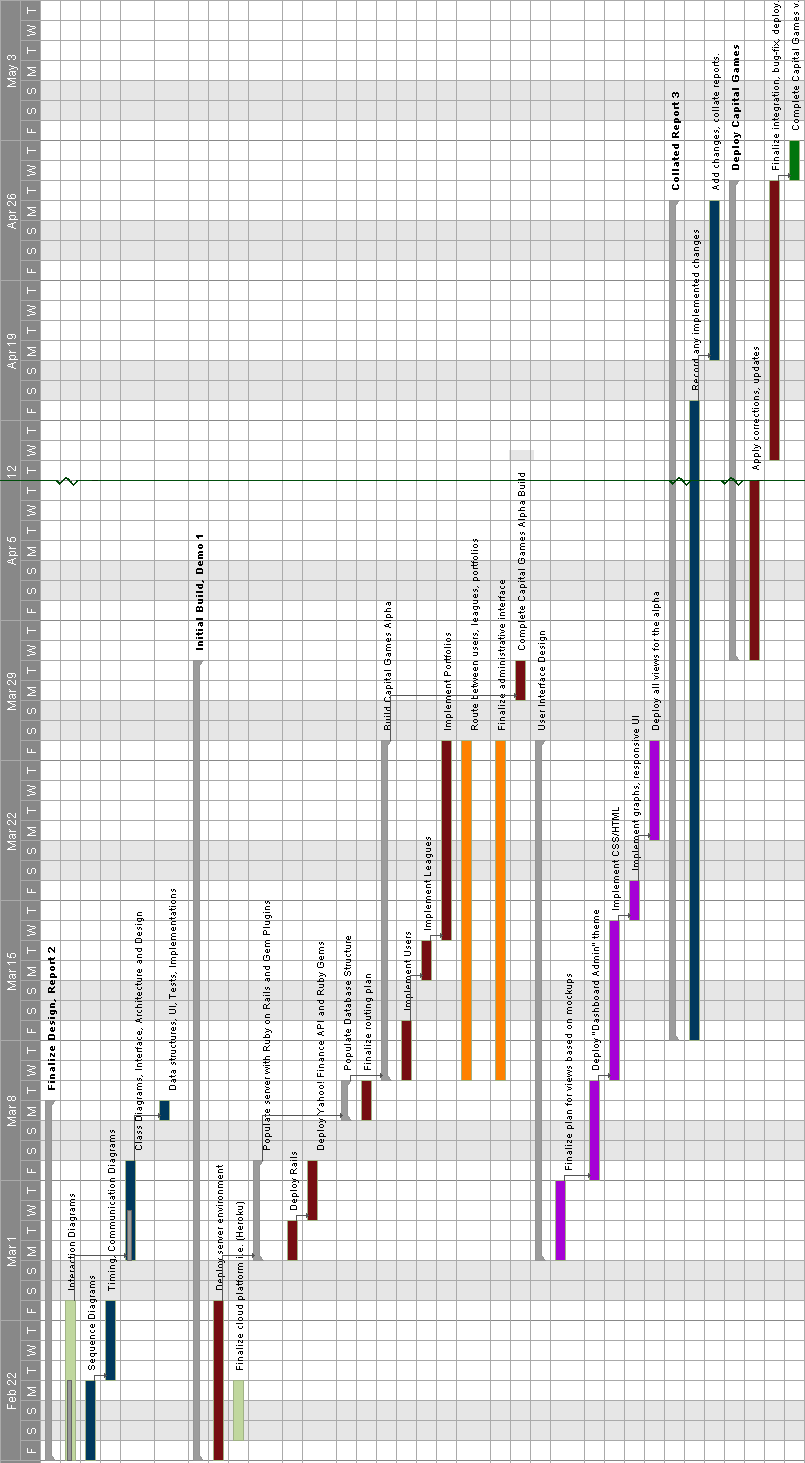
\includegraphics[width=6.5in]{./img/gantt.png}
\caption{This gantt chart projects how we will concurrently work on
the project. All blue items are report-related, red and orange relate
to the core project development and purple illustrates UI milestones.}
\end{figure}


%\section{User Story Matrix}
\section{Report 2 Contributions}
{
\begin{centering} % Aligns center 
\renewcommand\arraystretch{2} % Causes rows to be spaced slightly more
\begin{tabular}{cc|c|c|c|c|c|c|} % Creates a table with centered
                                 % columns "c", separated by bars "|"
\cline{3-8} % draw a horizontal line across columsn 3-8
& & \multicolumn{6}{ c| }{Names} \\ \cline{1-8}
\multicolumn{1}{|c|}{Category} & \multicolumn{1}{c|}{Points} & 
Jeff A & Eric C & Nick P & Jeff R & Val R & Dario R \\ \cline{1-8}
\multicolumn{1}{|c|}{UML Diagrams} & \multicolumn{1}{c|}{10 Points} & 
0\% & 0\% & 40\% & 50\% & 0\% & 10\% \\ \cline{1-8}
\multicolumn{1}{|c|}{Descr. of Diagrams} & \multicolumn{1}{c|}{10 Points} & 
20\% & 0\% & 0\% & 80\% & 0\% & 0\% \\ \cline{1-8}
\multicolumn{1}{|c|}{Alt. Solution Description} & \multicolumn{1}{c|}{10 Points} & 
0\% & 33\% & 0\% & 0\% & 33\% & 33\% \\ \cline{1-8}
\multicolumn{1}{|c|}{Class Diagram \& Description} & \multicolumn{1}{c|}{5 Points} & 
30\% & 10\% & 35\% & 0\% & 5\% & 20\% \\ \cline{1-8}
\multicolumn{1}{|c|}{Signatures} & \multicolumn{1}{c|}{5 Points} & 
0\% & 33\% & 0\% & 0\% & 33\% & 33\% \\ \cline{1-8}
\multicolumn{1}{|c|}{Styles} & \multicolumn{1}{c|}{5 Points} & 
25\% & 25\% & 10\% & 20\% & 20\% & 0\% \\ \cline{1-8}
\multicolumn{1}{|c|}{Package Diagram} & \multicolumn{1}{c|}{2 Points} & 
0\% & 0\% & 0\% & 0\% & 50\% & 50\% \\ \cline{1-8}
\multicolumn{1}{|c|}{Mapping Hardware} & \multicolumn{1}{c|}{2 Points} & 
0\% & 0\% & 0\% & 0\% & 50\% & 50\% \\ \cline{1-8}
\multicolumn{1}{|c|}{Database} & \multicolumn{1}{c|}{3 Points} & 
0\% & 0\% & 0\% & 0\% & 50\% & 50\% \\ \cline{1-8}
\multicolumn{1}{|c|}{Other} & \multicolumn{1}{c|}{3 Points} & 
0\% & 0\% & 0\% & 0\% & 50\% & 50\% \\ \cline{1-8}
\multicolumn{1}{|c|}{Algorithms \& Data Structures} & \multicolumn{1}{c|}{4 Points} & 
0\% & 0\% & 0\% & 0\% & 50\% & 50\% \\ \cline{1-8}
\multicolumn{1}{|c|}{Appearance} & \multicolumn{1}{c|}{6 Points} & 
0\% & 0\% & 0\% & 0\% & 50\% & 50\% \\ \cline{1-8}
\multicolumn{1}{|c|}{Prose Description} & \multicolumn{1}{c|}{5 Points} & 
0\% & 0\% & 0\% & 0\% & 50\% & 50\% \\ \cline{1-8}
\multicolumn{1}{|c|}{Testing Design} & \multicolumn{1}{c|}{12 Points} & 
0\% & 0\% & 0\% & 0\% & 50\% & 50\% \\ \cline{1-8}
\multicolumn{1}{|c|}{Document Merging} & \multicolumn{1}{c|}{11 Points} & 
0\% & 0\% & 0\% & 0\% & 50\% & 50\% \\ \cline{1-8}
\multicolumn{1}{|c|}{Project Coordination} & \multicolumn{1}{c|}{5 Points} & 
0\% & 0\% & 0\% & 0\% & 50\% & 50\% \\ \cline{1-8}
\multicolumn{1}{|c|}{Plan of Work} & \multicolumn{1}{c|}{2 Points} & 
0\% & 0\% & 0\% & 0\% & 50\% & 50\% \\ \cline{1-8}
\end{tabular}
\end{centering}
}